\chapter{Pianificazione}\label{Pianificazione}
Il gruppo \textit{Jawa Druids} ha pianificato le attività di progetto seguendo le scadenze riportate nel capitolo \ref{IntroduzioneScadenze}. Il progetto è dunque suddiviso nelle seguenti fasi:
\begin{itemize}
	\item Analisi;
	\item Consolidamento dei requisiti$_{\scaleto{G}{3pt}}$;
	\item Progettazione architetturale;
	\item Progettazione di dettaglio e codifica;
	\item Validazione e collaudo.
\end{itemize}
Ognuna di queste fasi è formata da attività$_{\scaleto{G}{3pt}}$ illustrate nei diagrammi di Gantt$_G$, che permettono la rappresentazione grafica di un calendario, utile al fine di pianificare, coordinare e tracciare specifiche attività dando una chiara illustrazione del suo stato di avanzamento.
Inoltre, considerato che queste fasi hanno una durata che varia da uno a due mesi, il gruppo ha deciso di suddividerle in periodi più brevi, elencando le attività da svolgere e gli incrementi previsti per tali periodi.
Le scadenze relative a questi periodi sono decise internamente dal Responsabile di Progetto dopo un consulto con il team.
\section{Analisi}\label{PianificazioneAnalisi}
\textbf{Periodo:} dal 22-10-2020 al 11-01-2021.\\
Questo periodo ha inizio con la formazione dei gruppi e la con la presentazione dei capitolati e termina con la scadenza per la consegna dei documenti relativi alla Revisione dei Requisiti.
Il lavoro svolto in questo periodo riguarderà principalmente l'analisi dei requisiti$_{\scaleto{G}{3pt}}$ posti dal proponente, la pianificazione, la scelta di metriche adeguate per il \textit{Piano di Qualifica} e la stesura della documentazione necessaria al supporto del progetto.
Tali compiti si possono identificare con le seguenti sette attività$_{\scaleto{G}{3pt}}$:
\begin{itemize}
	\item \textbf{Studio di Fattibilità:} attività$_{\scaleto{G}{3pt}}$ di studio di tutti i capitolati$_{\scaleto{G}{3pt}}$, elencando per ciascuno i punti positivi e negativi che li caratterizzano. Si specificano inoltre le motivazioni riguardanti la scelta del capitolato$_{\scaleto{G}{3pt}}$ \textit{GDP: Gathering Detection Platform}.
	Questa attività$_{\scaleto{G}{3pt}}$ è bloccante per l'inizio dell'\textit{Analisi dei Requisiti};
	\item \textbf{Norme di Progetto:} definisce tutte le regole, convenzioni e tecnologie che il gruppo \textit{Jawa Druids} deve rispettare ed utilizzare durante lo sviluppo dell'intero progetto;
	\item \textbf{Glossario:} racchiude termini che possono risultare ambigui durante lo svolgimento del progetto, con annessa una breve descrizione;
	\item \textbf{Piano di Progetto:} il presente documento in cui le attività$_{\scaleto{G}{3pt}}$, i compiti$_{\scaleto{G}{3pt}}$, e le risorse precedentemente analizzate vengono distribuite tra i componenti di \textit{Jawa Druids}. Presenta inoltre il calcolo del preventivo e le scadenze che il gruppo intende rispettare;
	\item \textbf{Lettera di Presentazione:} lettera in cui il gruppo \textit{Jawa Druids} si candida ufficialmente come fornitore$_{\scaleto{G}{3pt}}$ del prodotto software richiesto;
	\item \textbf{Analisi dei requisiti:} studio ed analisi dei requisiti$_{\scaleto{G}{3pt}}$ del capitolato$_{\scaleto{G}{3pt}}$ scelto nello \textit{Studio di Fattibilità};
	\item \textbf{Piano di qualifica:} documento in cui vengono indicate le strategie di verifica e validazione che il gruppo adotta per garantire la qualità del prodotto software.
\end{itemize}
\subsection{Primo periodo}\label{PianificazioneAnalisiPrimoPeriodo}
\textbf{22-10-2020 - 05-11-2020}: inizio dello \textit{Studio di fattibilità} attraverso l'analisi da parte di ogni membro del gruppo dei capitolati$_{\scaleto{G}{3pt}}$ proposti in modo da poterne discutere con gli altri membri per effettuare una scelta che mettesse d'accordo la maggioranza del gruppo.
Allo stesso tempo sono stati definiti alcuni aspetti tecnici riguardanti il gruppo come il nome, il logo e l'indirizzo email di riferimento.
\subsection{Secondo periodo}\label{PianificazioneAnalisiSecondoPeriodo}
\textbf{06-11-2020 - 06-12-2020}: inizio della stesura delle \textit{Norme di Progetto} dove vengono definite le regole per la stesura dei documenti e gli strumenti di supporto da utilizzare.
Studio dei ruoli di progetto con relativa assegnazione degli stessi ad ogni membro del gruppo, sarà il ruolo principale che ognuno ricoprirà durante l'intera fase di analisi.
Studio del resto della documentazione da produrre per la fine della fase, pianificazione della suddivisione del lavoro, definizione di scadenze da rispettare, studio dell'analisi dei rischi. Materiale che andrà a formare il \textit{Piano di Progetto}.
\subsection{Terzo periodo}\label{PianificazioneAnalisiTerzoPeriodo}
\textbf{07-12-2020 - 30-12-2020}: stesura dell'\textit{Analisi dei Requisiti} e del \textit{Piano di Qualifica} con l'esposizione delle metriche di qualità che nel frattempo saranno definite nelle \textit{Norme di Progetto}. Entro questo periodo il gruppo concluderà la stesura di tutti i documenti iniziati.
\subsection{Quarto periodo}\label{PianificazioneAnalisiQuartoPeriodo}
\textbf{31-12-2020 - 11-01-2021}: verifica di tutti i documenti di cui è terminata la stesura. Redazione del \textit{Glossario} e della lettera di \textit{Lettera di Presentazione}.
\subsection{Diagramma di Gantt: Analisi}\label{PianificazioneDiagrammaDiGanttAnalisi}
\begin{figure}[!h]
	\begin{center}
		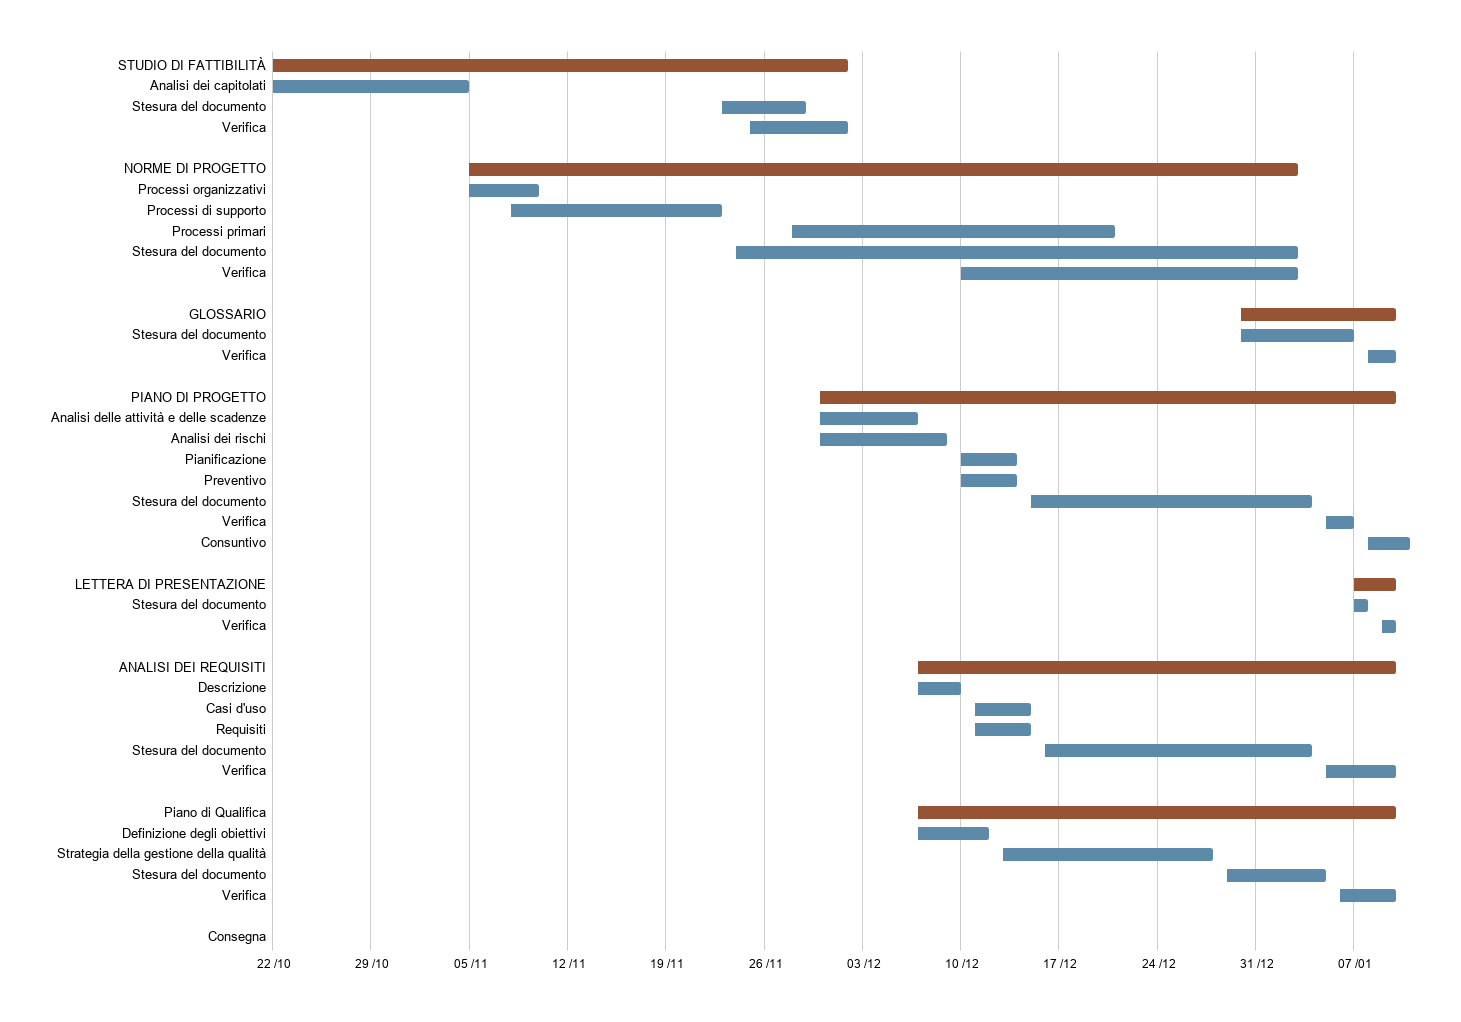
\includegraphics[width=1\linewidth]{../immagini/pdp/gantt_analisi.png}
		\caption{Diagramma di Gantt dell'attività di analisi}
	\end{center}
\end{figure}

\section{Consolidamento dei requisiti}\label{PianificazioneConsolidamentoDeiRequisiti}
\textbf{Periodo:} dal 11-01-2021 al 18-01-2021
Questo periodo ha inizio subito dopo il termine del precedente e finisce con la presentazione della Revisione dei Requisiti.
Il gruppo \textit{Jawa Druids} si dedicherà ai seguenti compiti$_{\scaleto{G}{3pt}}$:
\begin{itemize}
	\item avanzamento con lo studio individuale relativo a:
	\begin{itemize}
		\item acquisizione dei dati;
		\item simulazione dei dati;
		\item machine learning$_G$;
		\item web app.
	\end{itemize}
	\item preparazione del materiale necessario alla presentazione.
\end{itemize}
\subsection{Diagramma di Gantt: consolidamento dei requisiti}\label{PianificazioneDiagrammaDiGanttConsolidamento}
\begin{figure}[!h]
	\begin{center}
		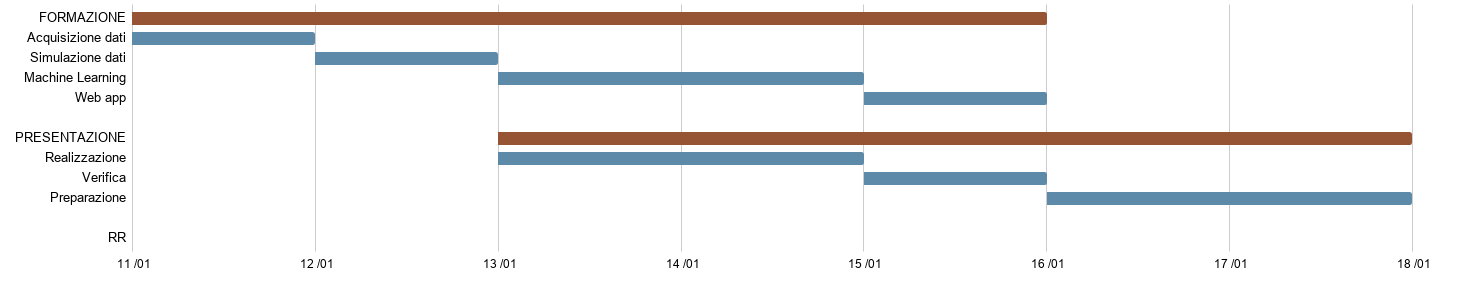
\includegraphics[width=1\linewidth]{../immagini/pdp/gantt_consolidamento_requisiti.png}
		\caption{Diagramma di Gantt del consolidamento dei requisiti}
	\end{center}
\end{figure}
\clearpage
\section{Progettazione architetturale}\label{PianificazioneProgettazioneArchitetturale}
\textbf{Periodo:} dal 19-01-2021 al 08-03-2021. \\
Questo periodo ha inizio subito dopo conclusione del precedente e termina con la Revisione di Progettazione.
Esso ha il compito di correggere ed incrementare la documentazione prodotta e di portare all'individuazione di una soluzione architetturale che permetta il soddisfacimento dei requisiti$_{\scaleto{G}{3pt}}$ obbligatori. È suddiviso in:
\begin{itemize}
	\item \textbf{Incremento e verifica:} analizzando l'esito della Revisione dei Requisiti, vengono svolte attività$_{\scaleto{G}{3pt}}$ di Incremento e Verifica sui vari documenti redatti, dove necessario;
	\item \textbf{Technology Baseline$_G$:} viene redatta la documentazione di supporto, contenente la descrizione delle tecnologie individuate e il tracciamento della relazione tra le componenti e i requisiti$_{\scaleto{G}{3pt}}$ che vanno a soddisfare.
	Viene realizzato un Proof of Concept$_G$ che verrà condiviso col proponente$_{\scaleto{G}{3pt}}$ per verificare il corretto sviluppo del software. In particolare il gruppo ha suddiviso ulteriormente questa fase in due incrementi:
	\begin{itemize}
		\item \textbf{Primo incremento -  15-02-2021 - 26-02-2021}: in questo periodo il gruppo svilupperà 5 moduli separati, ognuno riguardante un diverso aspetto del prodotto. In particolare i moduli 1 e 2 si occuperanno di ricavare il numero di persone presenti in un determinato luogo e istante di tempo partendo dal video di una webcam, produrranno in output un dato che conterrà tale informazione. Il modulo 3 dovrà prendere in input i dati che riceve dai moduli precedenti e salvarli nel database in modo da renderli disponibili per l'utilizzo. Il modulo 4 inizierà lo sviluppo di un modello di machine learning$_{\scaleto{G}{3pt}}$ in grado di fare previsioni future. Data la corposità di questo modulo, crediamo che questa funzionalità non sarà implementata nel Proof of Concept$_{\scaleto{G}{3pt}}$. Infine il quinto modulo si occuperà di prendere gli ultimi dati caricati nel database e visualizzarli in una heat map$_{\scaleto{G}{3pt}}$.
		\item \textbf{Secondo incremento - 27-02-2021 - 04-03-2021 }: nel periodo successivo il gruppo unirà tutti i prototipi dei moduli sviluppati in un unico Proof of Concept$_{\scaleto{G}{3pt}}$ che sia in grado di soddisfare alcuni dei casi d'uso$_{\scaleto{G}{3pt}}$ obbligatori. Tra questi il gruppo si pone come obiettivo che sia disponibile la heat map$_{\scaleto{G}{3pt}}$ (UC1) che prenda dati reali recentemente aggiunti al database (UC8.2), che vengano visualizzati i messaggi di errore in caso questi dati non siano disponibili (UC2 - UC9). Nel caso in cui ci sia la possibilità in termini di tempo, il Proof of Concept$_{\scaleto{G}{3pt}}$ continuerà ad essere sviluppato fino al termine della consegna, aggiungendo altri casi d'uso$_{\scaleto{G}{3pt}}$ obbligatori.
	\end{itemize}
\end{itemize}
\subsection{Primo Periodo}\label{PianificazioneProgettazioneArchitetturalePrimoPeriodo}
\textbf{19-01-2021 - 12-02-2021}: in questo primo periodo che, data la concomitanza con la sessione d'esami, risulta più esteso,  il gruppo inizierà la correzione dei documenti già redatti in concomitanza con la ricerca di fonti affidabili che ogni membro potrà consultare per fare formazione sulle tecnologie da utilizzare per la Technology Baseline$_{\scaleto{G}{3pt}}$.
\subsection{Secondo Periodo}\label{PianificazioneProgettazioneArchitetturaleSecondoPeriodo}
\textbf{13-02-2021 - 27-02-2021}: durante il secondo periodo il gruppo continuerà la propria formazione e deciderà come suddividere l'assegnazione dei moduli sopra citati. In seguito inizierà lo sviluppo degli stessi fino ad arrivare alla conclusione del primo incremento del Proof of Concept$_{\scaleto{G}{3pt}}$.
\subsection{Terzo Periodo}\label{PianificazioneProgettazioneArchitetturaleTerzoPeriodo}
\textbf{28-02-2021 - 08-03-2021}: in questo ultimo periodo il gruppo dovrà terminare anche il secondo incremento del Proof of Concept$_{\scaleto{G}{3pt}}$ ed ultimare la documentazione da presentare.

\subsection{Diagramma di Gantt: progettazione architetturale}\label{PianificazioneDiagrammaDiGanttProgettazioneArchitetturale}
\begin{figure}[h]
	\begin{center}
		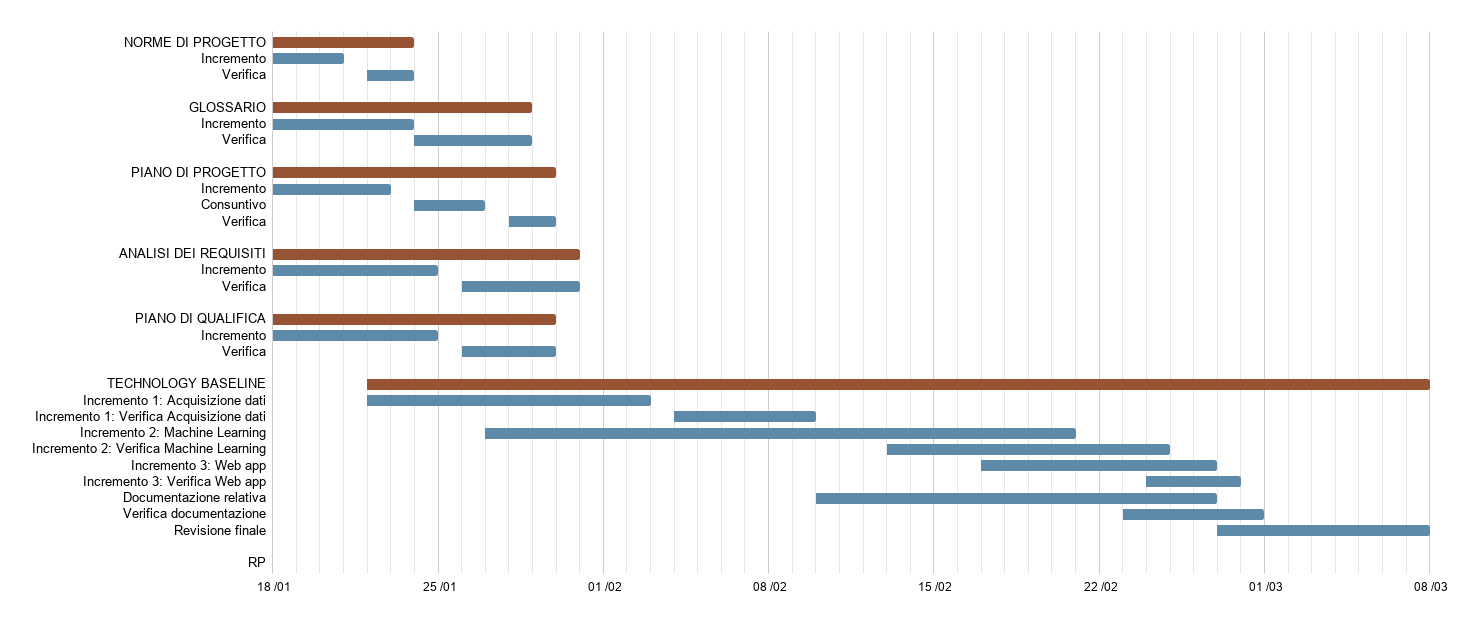
\includegraphics[width=0.9\linewidth]{../immagini/pdp/gantt_progettazione_architetturale.png}
		\caption{Diagramma di Gantt della progettazione architetturale}
	\end{center}
\end{figure}
\clearpage
\section{Progettazione di dettaglio e codifica}\label{PianificazioneProgettazioneDettaglio}
\textbf{Periodo:} dal 15-03-2021 al 09-04-2021
Questo periodo inizia appena concluso il precedente e termina con la Revisione di Qualifica.
Le principali attività$_{\scaleto{G}{3pt}}$ svolte in questo periodo sono
\begin{itemize}
	\item \textbf{Incremento e verifica:} alcuni dei documenti già prodotti vengono migliorati e aggiornati;
	\item \textbf{Product Baseline$_G$:} segue la Technology Baseline$_{\scaleto{G}{3pt}}$, dove vengono studiati meglio design pattern$_G$, classi e attività$_{\scaleto{G}{3pt}}$ necessarie alla codifica;
	\item \textbf{Specifica Tecnica:} è un documento contenente tutte le caratteristiche del prodotto e le motivazioni che hanno portato alla loro scelta;
	\item \textbf{Codifica:} attività$_{\scaleto{G}{3pt}}$ nella quale viene prodotto e verificato il codice;
	\item \textbf{Manuale utente:} attività$_{\scaleto{G}{3pt}}$ nella quale viene redatto il documento contenente le informazioni su come funziona e su come si utilizza il prodotto.
\end{itemize}
\subsection{Diagramma di Gantt: progettazione di dettaglio e codifica}\label{PianificazioneDiagrammaDiGanttProgettazioneDettaglio}
\begin{figure}[!h]
	\begin{center}
		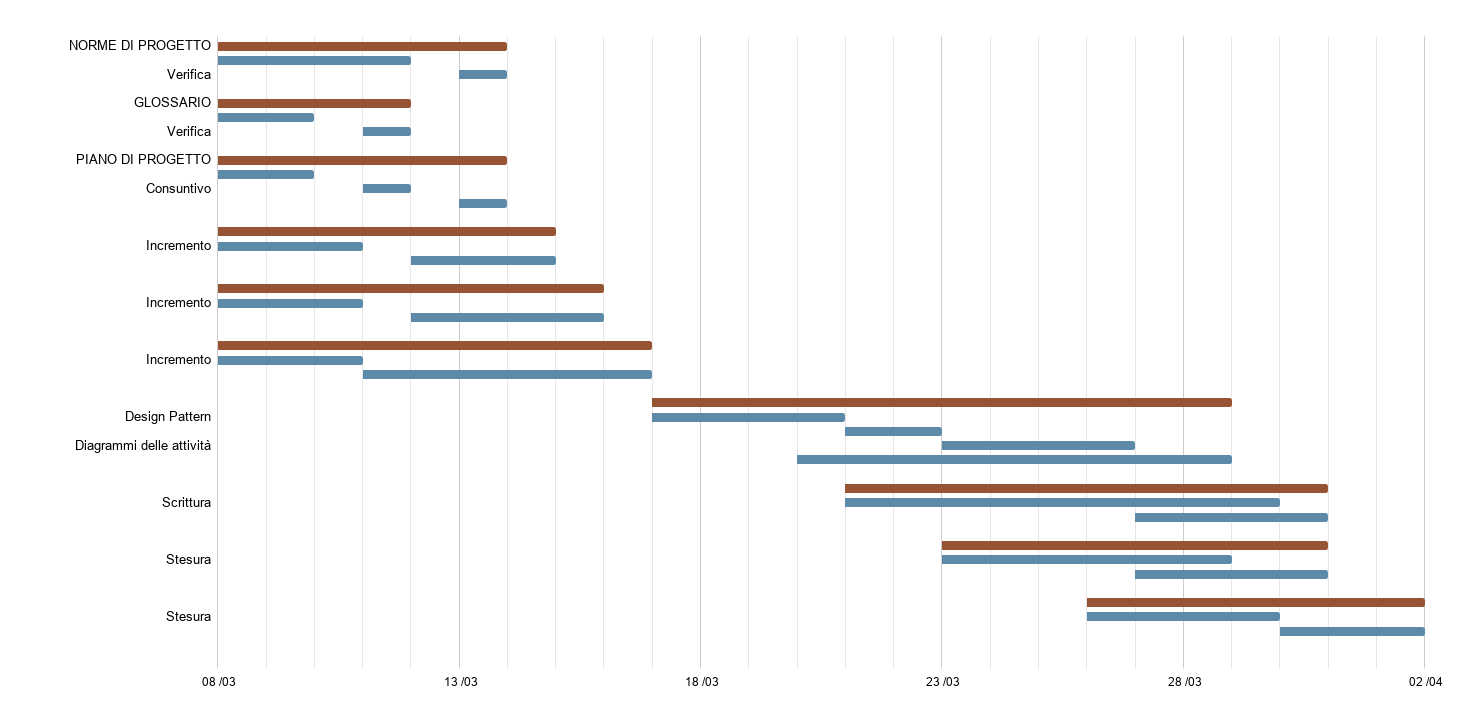
\includegraphics[width=0.8\linewidth]{../immagini/pdp/gantt_progettazione_dettaglio.png}
		\caption{Diagramma di Gantt dell'attività di progettazione di dettaglio e codifica}
	\end{center}
\end{figure}
\section{Validazione e Collaudo}\label{PianificazioneValidazione}
\textbf{Periodo:} dal 16-04-2021 al 10-05-2021
Questo periodo inizia appena concluso il precedente e termina con la Revisione di Accettazione.
Le principali attività$_{\scaleto{G}{3pt}}$ svolte in questo periodo sono:
\begin{itemize}
	\item \textbf{Incremento e verifica:} analizzando l'esito della Revisione di Qualifica vengono svolte attività$_{\scaleto{G}{3pt}}$ di Incremento e Verifica sui vari documenti redatti;
	\item \textbf{Validazione e Collaudo:} vengono realizzati gli ultimi test, con i dovuti controlli finali, in modo da garantire un buon livello di qualità e correttezza.
\end{itemize}
\subsection{Diagramma di Gantt: validazione e collaudo}\label{PianificazioneDiagrammaDiGanttValidazione}
\begin{figure}[!h]
	\begin{center}
		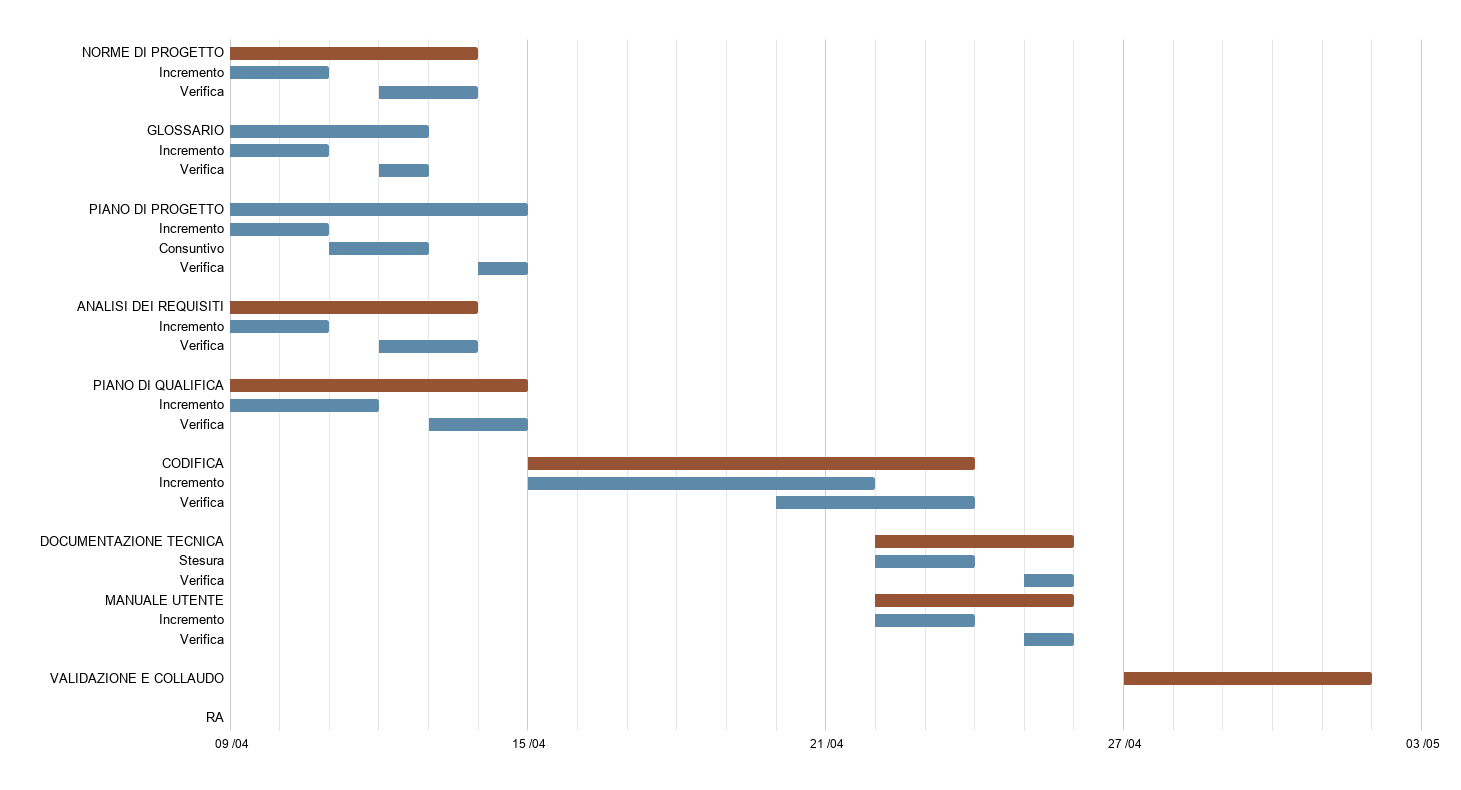
\includegraphics[width=0.8\linewidth]{../immagini/pdp/gantt_validazione.png}
		\caption{Diagramma di Gantt dell'attività di validazione e collaudo}
	\end{center}
\end{figure}
